\documentclass[14pt,a4paper]{extreport}

\usepackage{cmap}
\usepackage[T2A]{fontenc}
\usepackage[utf8]{inputenc}
\usepackage[english,russian]{babel}
\linespread{1.3}
\usepackage{indentfirst}
\usepackage{graphicx}
\usepackage{amsmath, amssymb, amsfonts}
\usepackage{array}
\usepackage{multirow}

\usepackage[a4paper, footskip=10mm,
            left=30mm, right=10mm, top=20mm, bottom=20mm]{geometry}

\graphicspath{ {./images/} }

\addto\captionsrussian{\renewcommand\chaptername{ГЛАВА}}
\addto\captionsrussian{\renewcommand\contentsname{ОГЛАВЛЕНИЕ}}


\makeatletter

% Оформление нумерованных глав
\renewcommand{\@makechapterhead}[1] {
  \vspace*{36pt} % Пустое место вверху страницы
  {
    \centering
    \parindent=18pt
    \Large\bfseries
    \chaptername ~ \thechapter{} \par % Номер главы
    #1 \par % Заголовок текста с новой строки
    \nopagebreak % Не отрываем заголовок от текста
    \vspace{36pt} % Пустое место между заголовком и текстом
  }
}

% Оформление ненумерованных глав
\renewcommand{\@makeschapterhead}[1] {
  \vspace*{36pt} % Пустое место вверху страницы
  {
    \centering
    \parindent=18pt
    \Large\bfseries #1 \par
    \nopagebreak % чтобы не оторвать заголовок от текста
    \vspace{25pt} % между заголовком и текстом
  }
}

\makeatother


\begin{document}
\begin{titlepage}
\begin{center}
    \small
    \textbf{МИНИСТЕРСТВО ОБРАЗОВАНИЯ РЕСПУБЛИКИ БЕЛАРУСЬ}
    \vspace{0.25cm}

    \textbf{БЕЛОРУССКИЙ ГОСУДАРСТВЕННЫЙ УНИВЕРСИТЕТ}
    \vspace{0.25cm}

    \textbf{ФАКУЛЬТЕТ ПРИКЛАДНОЙ МАТЕМАТИКИ И ИНФОРМАТИКИ}
    \vspace{0.25cm}

    \normalsize
    \textbf{Кафедра биомедицинской информатики}
    \vfill

    \textbf{СОЗДАНИЕ БАЗЫ ИЗОБРАЖЕНИЙ УЧАСТКОВ ЗЕМНОЙ ПОВЕРХНОСТИ И ОБУЧЕНИЕ
    СВЁРТОЧНОЙ НЕЙРОННОЙ СЕТИ ДЛЯ ИХ РАСПОЗНАВАНИЯ С БОРТА ДРОНА}
    \vfill

    Курсовая работа

\end{center}
\vfill

\hfill\begin{minipage}{0.5\textwidth}
    Калабука Дмитрия Сергеевича\\
    студента 3 курса,\\
    специальность <<Информатика>>
    \vspace{0.25cm}

    Научный руководитель:
    Ковалёв В.А.
\end{minipage}
\bigskip


\begin{center}
    Минск, 2018
\end{center}

\end{titlepage}



\newpage
\tableofcontents

\newpage
\addcontentsline{toc}{chapter}{ВВЕДЕНИЕ}
\chapter*{ВВЕДЕНИЕ}
Сегментация изображения --- это разделение изображения на области, однородные по
некоторому критерию. Сегментация, при которой области разбиения не пересекаются,
называется \textit{тесселяцией}. Цель сегментации состоит в упрощении или
изменении представления изображения для последующей интерпретации содержимого на
изображении.
Результатом сегментации является множество сегментов, которые
покрывают все изображение. Иначе говоря, каждый пиксель отмечен меткой
некоторого класса. На сегодняшний день известно большое количество алгоритмов
сегментации изображений, использующих разные подходы. Многие из них являются
нейросетевыми. Для обучения таких алгоритмов нужно большое количество
подготовленных данных. Кроме того, при исследовании подходов к решению задачи
сегментации изображений возникает задача оценки качества выбранного алгоритма
для сравнения его с другими подходами.  Таким образом, для решения задачи
сегментации необходимо:
\begin{itemize}
    \item Найти и подготовить данные для анализа.
    \item Разработать алгоритм сегментации для полученных данных.
    \item Выбрать критерий для оценки качества алгоритма сегментации.
\end{itemize}

Сегментация изображений находит широкое применение в поиске аномалий на
медицинских изображениях, в выделении объектов на спутниковых снимках, в
системах управления дорожным движением, распознавании лиц, распознавании
отпечатков пальцев, в подготовительных работах для анализа текста на
изображении, в сельском хозяйстве, и т.д.  В данной работе задача сегментации
изображений применяется для выявления различных классов на изображении земной
поверхности.  Особенность задачи сегментации изображений земной поверхности
заключается в том, что параметры изображения зависят от многих факторов, таких
как время года, время суток, в которое был сделан снимок, угол наклона к
поверхности земли. У разных поставщиков изображения заметно отличаются.  На
практике далеко не всегда есть возможность получить изображения всех
встречающихся типов, поэтому возникает задача обучения алгоритма на одном типе
данных (например, на изображениях одного поставщика) таким образом, чтобы он был
применим и давал приемлимые результаты на данных других типов.
%image

\newpage
\section*{Поставленные задачи}
\begin{itemize}
    \item Подготовить базу изображений снимков земной поверхности.
    \item Разметить данные, то есть для каждого изображения создать ``маску'', где
        указан номер класса для каждой области.
    \item
        Опробовать различные подходы решения задачи сегментации.
    \item Обучить полносвязную конволюционную сеть для семантической
        сегментации.
    \item Сравнить различные методы решения проблемы вариативности данных.
    \item Научиться использовать источник OpenStreetMap для получения
        размеченных данных.
    \item Исследовать применимость данных OpenStreetMap для обучения алгоритмов
        сегментации земной поверхности.
\end{itemize}


\newpage
\chapter{АЛГОРИТМЫ КЛАССИФИКАЦИИ}
В качестве базовой оценки качества исследуемых алгоритмов предлагалось
использовать точность основных алгоритмов машинного обучения, выполняющих
классификацию изображений. В качестве таких алгоритмов использовались SVM, KNN,
Random Forest. Как и большинство алгоритмов классификации, они требуют, чтобы их
входом были точки (объекты) в $M$-мерном пространстве, а выходом является
число --- номер класса, или по одному числу в интервале $[0, 1]$ на каждый
класс --- вероятности того, что объект лежит в данном классе. Поэтому из каждого
исходного изображения были вырезаны квадраты $64 \times 64$ пикселя, в которых
больше $90\%$ площади принадлежат одному классу.  Классом изображения считается
преобладающий класс пикселей. Для представления таких изображений в виде точек
(векторов признаков) использовались различные дескрипторы.


\section{Классические алгоритмы}
Рассмотрим использованные алгоритмы машинного обучения подробнее.

\subsection{Linear SVM}
В случае двух классов предполагает, что выборка линейно разделима, т. е.
существует гиперплоскость, разделяющая всё пространство $\mathbb{R}^M$ на два
полупространства таких, что объекты, принадлежащие разным классам, лежат в
разных полупространствах. При этом из всех возможных разделяющих гиперплоскостей
выбирается та, которая наиболее удалена от объектов обоих классов.  В случае
нескольких классов рассматривается каждая пара классов, определяется
принадлежность классу из пары, а затем производится усреднение результатов для
получения предсказания номера класса

\subsection{K Nearest Neighbors}
Для определения класса данного объекта рассматриваются $K$ объектов из обучающей
выборки (для которой известны ответы), находящиеся ближе всего к данному объекту
по какой-то заранее заданной метрике в пространстве $\mathbb{R}^M$. В качестве
ответа для объекта используется класс, к которому принадлежит большинство из
найденных ``соседей''. В данной работе использовался параметр K равный $1$,
потому что он показывал лучший результат при экспериментах.

\subsection{Random Forest}
Использует голосование решающих деревьев. Каждое дерево в каждой своей вершине
пытается разделить множество объектов по, так называемому, решающему правилу,
которое использует какое-то небольшое подмножество признаков. При помощи
различных эвристик решающее правило выбирается так, чтобы разделять классы как
можно более равномерно. Полученные подмножества разделяются более глубокими
вершинами дерева. В листьях хранится ответ. Как правило, это самая частая метка
класса из множества объектов обучающей выборки, попавших в этот лист.
Преимуществами является способность классифицировать линейно неразделимую
выборку. Для всех экспериментов использовалось $75$ решающих деревьев, т.к. это
значение давало довольно хороший результат при приемлимом времени обучения.


\section{Дескрипторы}
Для преобразования изображений $64 \times 64$ пикселя в точки в $\mathbb{R}^M$
использовались следующие дескрипторы.

\subsection{Гистограмма яркостей}
Сначала изображение преобразуется в чёрно-белое. Затем спектр яркостей
$[0, 255]$ делится на $16$ равных отрезков: $[0, 15], [16, 31], \ldots, [240,
255]$. Для каждого отрезка вычисляется количество пикселей изображения, яркость
которых находится в соответствующем этому отрезку диапазоне. Полученные $16$ чисел
являются признаками, т. е. координатами точки, соответствующей данному
изображению.

\subsection{Гистограмма независимых цветов}
Указанные выше $16$ признаков считаются для каждого из трёх каналов изображения
(каждый из которых можно представлять как чёрно-белое изображение) и
конкатенируются. Недостатком такого подхода является то, что каналы изображения
считаются независимыми, а значит преобразование одного из каналов, которое не
изменит дескриптор, может сильно изменить цвета изображения. Очевидно, что такой
подход даёт плохие результаты, и почти не используется на практике.

\subsection{Кластеризация цветов}
Цвета представляются как точки в трёхмерном пространстве. Выбирается количество
кластеров $K$. В данной работе проводились эксперименты с количеством кластеров
32, 64 и 128. Все цвета, встречающиеся во всех изображениях разделяются на
выбранное количество кластеров алгоритмом K-Means, запоминаются центроиды
(центры масс) каждого кластера. Затем для данного изображения и каждого номера
кластера подсчитывается, сколько пикселей относятся к этому кластеру. Считается,
что пиксель относится к кластеру, если он удалён от центроида этого кластера
меньше, чем от центроидов всех остальных кластеров. Получается $K$ признаков для
каждого изображения. Т.к. количество пикселей на всех изображениях очень
большое, для кластеризации используется случайное их подмножество.


\section{Метрики}
Во всех экспериментах в качестве метрики использовалась \textit{точ\-ность}
(англ. \textit{ac\-cu\-ra\-cy}) --- доля правильно предсказанных изображений из всех. У
такой метрики есть недостатки. Например, иногда на практике ошибки в одних
классах более критичные, чем другие. Также при большом количестве классов
алгоритм может вовсе не научиться определять один из них, но при этом иметь
хорошую точность засчёт корректного определения других. Для наших целей эта
метрика была достаточно показательной.


\section{Результаты классических алгоритмов}
Для сравнения алгоритмов и дескрипторов была измерена точность классификации
изображений. Алгоритмы обучались на некоторых размеченных данных. Затем
проводились измерения качества на данных того же поставщика. В таблице
\ref{table:classical_algo__comparison} приведены полученные значения точности.

\begin{table}[ht]
\caption{Сравнение классических алгоритмов и дескрипторов}
\label{table:classical_algo__comparison}
\small
\begin{tabular}{|m{68mm}|m{26mm}|m{26mm}|m{28mm}|}
    \hline
    & LinearSVM & KNN & RandomForest\\
    \hline
    Гистограмма яркостей           & $0.851$ & $0.883$ & $0.920$\\
    \hline
    Гистограмма независимых цветов & $0.879$ & $0.903$ & $0.927$\\
    \hline
    Кластеризация, $32$ кластера   & $0.906$ & $0.900$ & $0.940$\\
    \hline
    Кластеризация, $64$ кластера   & $0.883$ & $0.902$ & $0.940$\\
    \hline
    Кластеризация, $128$ кластера  & $0.896$ & $0.898$ & $0.934$\\
    \hline
\end{tabular}
\end{table}

Также были проведены эксперименты по обучению и проверке качества на различных
поставщиках. Результаты (значения точности) приведены в таблице
\ref{table:providers_comparison}.

\begin{table}[ht]
\caption{Результаты при обучении на данных разных поставщиков}
\label{table:providers_comparison}
\small
\begin{tabular}{|r|r|m{22mm}m{22mm}m{22mm}m{22mm}|}
    \hline
         &        & \multicolumn{4}{|c|}{Поставщик для оценки качества}\\
    \hline
         &        & Google  & Yandex  & Bing    & ESRI\\
    \hline
    \multirow{4}{24mm}{Поставщик для обучения}
         & Google & --      & $0.819$ & $0.956$ & $0.840$\\
         & Yandex & $0.432$ & --      & $0.843$ & $0.861$\\
         & Bing   & $0.754$ & $0.915$ & --      & $0.960$\\
         & ESRI   & $0.593$ & $0.908$ & $0.988$ & --\\
    \hline
\end{tabular}
\end{table}

В результате этого эксперимента стало понятно, что между изображениями различных
поставщиков существуют значительные различия, что заметно влияет на качество
классификации. В дальнейшем использовались разные подходы для устранения этой
проблемы.


\section{Нейросетевые алгоритмы}
Нейросетевыми называются такие вычислительные системы, которые обладают
способностью к самообучению и постепенному повышению производительности. Они
используются при решении таких задач, которые не поддаются логическому
программированию. Таковыми являются многие задачи анализа и обработки
изображений, в том числе задача классификации изображений.
В задачах связанных с изображениями чаще всего применяются \textit{свёрточные
нейронные сети} (англ. \textit{convolutional neural networks}). В основе таких
сетей лежит операция свёртки матриц. Такие сети позволяют использовать меньше
нейронов по сравнению с сетями использующими полносвязные слои, и обладают
свойством локальности --- результаты работы сети слабо подвержены таким
изменениям как перемещение целевого объекта на изображении.

Одной из известных архитектур свёрточной нейронной сети для классификации
является архитекрута VGG \cite{vgg}. Основное её отличие от других свёрточных сетей ---
замена слоёв с фильтрами $n \times n$ на комбинацию слоёв $3 \times 3$. Такой
подход даёт примерно такие же возможности классификации, но задействуется меньше
обучаемых весов, что способствует более быстрому обучению и лучшему качеству
сети. Например, фильтр $5 \times 5$ использует $25$ связей (и, соответственно,
весов), а два слоя $3 \times 3$ обладают тем же рецептивным полем, но суммарно
используют $18$ связей.
Рецептивное поле --- окрестность в предыдущем слое
нейросети, значения которой влияют на значение фиксированного нейрона в текущем
слое.  Ещё одной особенностью архитектуры VGG является увеличение числа
свёрточных фильтров в $2$ раза по сравнению с предыдущим слоем.

Использованная нейронная сеть состоит из $5$ свёрточных уровней и двух
полносвязных слоёв. Каждый уровень состоит из двух свёрточных слоёв с фильтрами
$3 \times 3$, слоя активации (ReLU) и MaxPooling слоя. MaxPooling --- это слой,
уменьшащий размер карты признаков путём замены каждой окрестности $2 \times 2$
пикселя на $1$ число --- максимум чисел в этой окрестности.

Для работы с многоклассовыми данными используется one-hot-encoding --- метки
классов для каждого пикселя в ответе заменяются на вектор, длина которого
равна количеству классов. В этом векторе на позиции, соответствующей номеру
класса, стоит $1$, а на остальных --- $0$. Последний полносвязный слой сети
состоит из числа нейронов равного числу классов изобажений. Результатом работы
алгоритма на изображении является вектор, длина которого равна числу классов,
--- вероятности классов (степени уверенности алгоритма в принадлежности
изображения данному классу). 

Для решения проблемы вариативности данных была использована \textit{аугментация}
(англ.  \textit{augmentation}) --- небольшое случайное изменение входных
изображений во время обучения так, чтобы класс, которому принадлежит изображение
остался прежним. Аугментация позволяет имитировать вариативность выборки, не
проделывая дополнительную работу по подготовке данных. Такой приём повысил
точность с $78\%$ до $82\%$.


\newpage
\chapter{АЛГОРИТМЫ СЕГМЕНТАЦИИ}
В отличие от задачи классификации, задача сегментации заключается в разделении
изображения на области, принадлежащие одному классу. В такой задаче
предсказываемым ответом (маской) будет изображение такого же размера, как
исходное, но пиксели в нём будут обозначать не цвета, а номер класса, которому
принадлежит соответствующая позиция на исходном изображении.

Рассмотрим несколько различных подходов к решению задачи сегментации
изображений.

\addcontentsline{toc}{section}{Разбиение изображения на части}
\section*{Разбиение изображения на части}
Это один из самых простых в понимании и реализации подход. Изображение делится
на достаточно маленькие, возможно пересекающиеся, части квадратной формы. Но
достаточно большие, чтобы можно было по такой части изображения без контекста
определить, к какому классу она относится. Для простоты реализации все части
делаются одинакового размера. Затем решается задача классификации изображений,
т.е. разрабатывается алгоритм, который каждому маленькому изображению ставит в
соответствие число --- номер класса. Для обучения такого алгоритма из
размеченных исходных изображений выбираются такие части нужного размера, в
которых доля пикселей относящихся к одному классу больше заранее выбранного
порога, например, 95\%. После классификации каждой части, требуется восстановить
маску классов целого изображения, т.е. поставить в соответствие каждому пикселю
предполагаемый номер класса. В случае, если изображение разбивалось на
непересекающиеся части, считается, что каждый её пиксель относится к тому
классу, к которому была отнесена эта часть. Если же части пересекались, то такая
раскраска производится только с центральной областью достаточного размера каждой
части.

\addcontentsline{toc}{section}{Полноконволюционные нейронные сети}
\section*{Полноконволюционные нейронные сети}
Более подходящими и используемыми методами для решения задачи сегментации
являются нейросетевые методы. Т.к. в задаче сегментации нужно получать не число,
а целое изображение, то требуется использовать более сложную структуру сети, чем
классические свёрточные сети.

Базовые единицы в полноконволюционных сетях --- всё те же свёрточные слои. Но в
них не используюся полносвязные слои.  Полноконволюционная сеть состоит из двух
частей --- \textit{Encoder} и \textit{Decoder}. Encoder состоит из тех же
свёрточных слоёв, слоёв активации и MaxPooling слоёв. При проходе через Encoder
размер карты признаков уменьшается (но, возможно, увеличивается количество слоёв
карты признаков). Слои в decoder иногда называют \textit{деконволюционными},
т.к. проходя через decoder размер карты признаков увеличивается, пока не станет
такого же размера как исходное изображение. Но в действительности в части
decoder используются обычные свёрточные слои, обычно $3 \times 3$ и функция
активации. Только слои MaxPooling заменяются на слои UpSampling. Каждой точке
карты признаков они ставят в соответствие квадрат $2 \times 2$ со значением этой
точки. Именно эти слои увеличивают размер карты признаков.

Основным преимуществом такой сети являеся то, что её архитекрута не зависит от
размера входных изображений. Т.е. на вход могут подаваться изображения различных
размеров (но не слишком маленьких), и сеть сможет обрабатывать любые из них
с помощью фиксированного набора обученных весов.

Для экспериментов была выбрана архитекрута UNet. В ней в каждом слое части
decoder помимо выхода предыдущего слоя используется также карта признаков части
encoder такого же размера. Используются те же уровни, что и в VGG --- пары
свёрточных слоёв с фильтром $3 \times 3$, ReLU и MaxPooling или UpSampling.
С помощью этого алгоритма удалось достичь точность $88\%$, применяя его к
исходным данным, и $93\%$, если применять методы борьбы с вариативностью данных,
о чём будет написано дальше. % TODO
Часть полученного результата показана на рисунке \ref{fig:segm_result}

\begin{figure}[p]
    \centering
    \caption{Результат сегментации изображения}
    \label{fig:segm_result}
    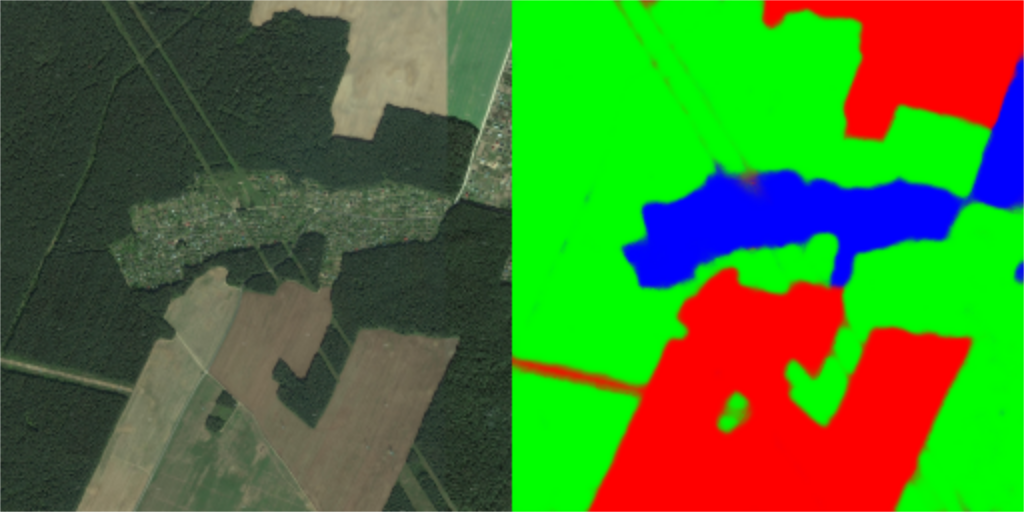
\includegraphics[width=0.8\textwidth]{images/segm_results_yandex.png}
\end{figure}

\addcontentsline{toc}{section}{Метрика IoU}
\section*{Метрика IoU}
Для оценки результатов сегментации, помимо точности, можно посчитать ещё одну
довольно информативную метрику --- \textit{Intersection over Union}
(\textit{IoU}). Она вычисляется для бинарных изображений, т.е. тех, где каждый
пиксель отнесён к одному из двух классов. Поэтому изображения карты вероятностей
нужно сначала обрезать по какому-либо порогу $T$. Т.е. заменить значения меньше
$T$ на $0$, а больше $T$ --- на $1$. Затем два сравниваемых изображения
(истинная маска и результат работы алгоритма) рассматриваются как множества
точек, в которых находятся $1$. Пусть это множества $A$ и $B$ (порядок не
важен). Тогда значение $\Omega$ метрики IoU равно
$$
\Omega = \frac{A \cap B}{A \cup B}
$$
Чем ближе значение $\Omega$ к $1$, тем лучше качество сегментации.


\newpage
\chapter{ПОДГОТОВКА ДАННЫХ}
Итак, самым подходящим подходом к решению задачи сегментации является
использование нейронных сетей. Их особенностью является то, что для достижения
хорошего результата им требуется большой объём данных для обучения. Сейчас в
свободном доступе есть большое число поставщиков космических изображений всей
поверхности земли.  Например, Yandex, Google, Bing, ESRI Imagery, и т. д.
Поэтому получение неразмеченных данных не является проблемой. Для обучения
алгоритмов классификации и сегментации необходима ``разметка'' данных, т. е.
информация о классах, которые алгоритм должен научиться распознавать. Для
дальнейшей работы требовалось выполнить разметку имеющихся данных. Для каждого
региона, из которого получены изображения составлялся файл ``маски'' этого
региона, состоящий из одноцветных областей, цвет которых обозначает какой-то
класс. Выполнение этого вручную требует значительных затрат человеческих сил и
времени. Поэтому было решено попробовать использовать размеченные данные, уже
существующие в открытом доступе.


\addcontentsline{toc}{section}{Использование данных OpenStreetMap}
\section*{Использование данных OpenStreetMap}
OpenStreetMap (OSM) – проект по созданию подробной свободной и бесплатной
географической карты мира. Карты OSM уже содержат в себе подробную информацию о
многих регионах земной поверхности. Информация добавляется и редактируется
добровольцами во всех странах мира. Вся информация в OSM хранится в векторном
виде.  Данные делятся на несколько типов:
\begin{enumerate}
    \item \textit{Точки} (\textit{Nodes})
    \item \textit{Линии} (\textit{Ways})
    \item \textit{Замкнутые линии} (\textit{Closed ways})
    \item \textit{Заполненные области} (\textit{Areas})
    \item \textit{Отношения} (\textit{Relations})
\end{enumerate}
С сайта OSM можно скачать данные в векторном виде. В них будут содержаться
данные указанных типов, с пометками о типе региона, из которых можно определить,
является ли участок полем/застройкой/водным ресурсом и т. д.
Чтобы получить данные в формате, требуемом для обучения описанных ранее
алгоритмов, нужно было их растеризовать. Для этих целей использовалась утилита
\textit{gdal\_rasterize}.
Использование готовой разметки из такого источника как OpenStreetMap значительно
упрощает работу по подготовке данных для обучения.

Далее, чтобы не отвлекаться на пролемы связанные с алгоритмами многоклассовой
сегментации, было решено рассматривать бинарную классификацию для исследования
применимости данных OSM для разметки изображений. В качестве классов были взяты
постройки и фон, т.е. всё, что не является постройками. Такое решение было
сделано в том числе потому что постройки размечаются в OSM чаще и более
качественно, чем, например, поля. Вероятно, так происходит потому что большую
часть аудитории OSM интересуют именно карты городов и поселений.
Было создано более $20$-ти размеченных изображений с размерами от $3000$ до
$8000$ пикселей. После проведения сегментации этих изображений, была достигнута
примерно такая же точность, что и при многоклассовой сегментации. Значение IoU
варьировалось от $0.3$ до $0.5$.
Но при просмотре результатов оказалось, что сеть недостаточно чётко распознавала
границы зданий. Выяснилось, что данных OSM разметка зачастую сдвинута достаточно
сильно, чтобы не проходить по границе здания. Причём разметка разных зданий
сдвинута в разные стороны, т.е. природа этой погрешности является случайной.
Для количественного измерения этой погрешности для одного из изображений была
проведена аккуратная ручная разметка. Значение IoU между OSM и ручной разметкой
составило $0.631$, что меньше, чем хотелось бы ожидать от алгоритма сегментации.

Таким образом, было решено, что данные OSM в чистом виде не подходят для
использования в качестве сегментационной маски. Но были получены и полезные
результаты. Даже при обучении не сдвинутых масках, алгоритм научился
детектировать здания достаточно хорошо, чтобы находить не изображениях те здания,
которые не были размечены в данных OSM. При правильном использовании это может
принести практическую пользу.


\addcontentsline{toc}{section}{Проблема вариативности данных}
\section*{Проблема вариативности данных}
Как уже было отмечено, данные различных поставщиков отличаются довольно сильно.
Засчёт этого, при обучении алгоритма на данных одного поставщика и попытке
сделать предсказание на данных другого поставщика (возможно, даже той же
местности) результаты получаются неудовлетворительными, намного хуже, чем при
обучении и тестировании на данных одного поставщика. Такой эффект называется
\textit{переобучением}. Аугментация --- один из подходов, признанных частично
избавиться от такого неблагоприятного эффекта. Но она не является решением всех
проблем.

Одно из заметных отличий данных разных поставщиков --- различные цветовые
палитры изображений. Существует подход, позволяющий привести цвета на
изображении к некоторой канонической палитре с целью сблизить цветовую разницу
даже тех изображений, у которых палитры сильно отличаются. Идея заключаетяс в
том чтобы нормализовать цвета в окрестности каждой точки. Т.е. из яркости
каждого канала каждой точки вычитается средняя яркость этого канала у всех точек
в окрестности некоторого фиксированного радиуса, и полученное значение делится
на корень из дисперсии яркостей этого канала у пикселей в той же окрестности.
После такого преобразования все изображения состоят из цветов близких к серому,
но границы сохраняются, и объекты на изображении всё ещё отличимы. Такой подход
давал некоторый прирост качества алгоритма, но он практически не совместим с
аугментацией, которая давала больший прирост качества.

Существуют принципиально другие, более мощные алгоритмы, позволяющие перейти от,
так называемого, \textit{домена} одного изображения к домену другого. Сами эти
алгоритмы основываются на нейронных сетях и используют в своей основе Generative
Adversarial Networks. Если научиться переводить изображения любого поставщика в
домен изображений поставщика, на которых производилось обучение, то качество
должно быть таким же хорошим как при тестировании алгоритма на тех изображениях,
на которых он обучался. Идея в том, что для тренировки алгоритма доменной
адаптации не нужны размеченные изображения, а достаточно любых изображений обоих
поставщиков. В рамках данной работы не проводились исследования в этом
направлении.


\end{document}
